\documentclass[12pt]{article}
\setlength{\oddsidemargin}{0in}
\setlength{\evensidemargin}{0in}
\setlength{\textwidth}{6.5in}
\setlength{\textheight}{8.0in}
\setlength{\parindent}{0in}
\setlength{\parskip}{\baselineskip}

\usepackage{tikz}
\usepackage{hyperref}
\usetikzlibrary {arrows.meta,bending,positioning,quotes,shapes.geometric,bayesnet,calc}
\usepackage{color,calc,enumerate,tabu,graphicx,multicol,fullpage,amssymb,bm, float}
\usepackage{soul}

\setlength{\headheight}{16pt}
\newlength\longanswerwidth
\setlength{\longanswerwidth}{\textwidth-0.8cm}
\newcommand{\mycolumnwidth}{13cm}
\newcommand{\answerbox}[2]{\fbox{\begin{minipage}{#1}\hfill\vspace{#2}\end{minipage}}}
\newenvironment{qparts}{\begin{enumerate}[{(}a{)}]}{\end{enumerate}}
\newenvironment{qsubparts}{\begin{enumerate}[{(}i{)}]}{\end{enumerate}}

\usepackage{fancyhdr}
\setlength{\headheight}{16pt}


\title{Assignment 4}

\begin{document}

% Set up a footer for all pages, with student name, number, and page number:
\pagestyle{fancy}
\fancyhead{}
\renewcommand{\headrulewidth}{0pt} % no line in header area
\fancyfoot{}
\fancyfoot[L]{\textcolor{blue}{Alexandre Labbé}, student number \textcolor{blue}{2377032}}
\fancyfoot[R]{\thepage}

{\huge \bf CSE 415 Winter 2024\hfill Assignment 4}  \\
\vspace{0.2cm}

{\textcolor{blue}{}}\\

% Although it's also in the page footers, put your name here to show up prominently on the first page:
Last name: {\textcolor{blue}{Labbé}} \hspace{1cm} First name: {\textcolor{blue}{Alexandre}} \hfill  \\
\vspace{0.2cm}

This is an individual-work assignment. Do not collaborate on
this assignment.

Prepare your answers in a neat, easy-to-read
PDF. Our grading rubric will be set up such that
when a question is not easily readable
or not correctly tagged or with pages repeated or
out of order, then points will be
be deducted.  However, if all answers are
clearly presented, in proper order, and
tagged correctly when submitted to Gradescope,
we will award a 5-point bonus. (Thus the maximum points for A4 will be 105.)

If you choose to choose to typeset your answers
in Latex using the template file for this document,
please put your answers in \textcolor{red}{blue} while
leaving the original text black.

\hrulefill
\vspace{0.2cm}
\newpage
\section{Basic Search}

Use the following tree to answer the questions below comparing Breadth First Search, Depth First Search, and Iterative-Deepening Depth First Search. Assume that children are visited from left to right.

\begin{center}
  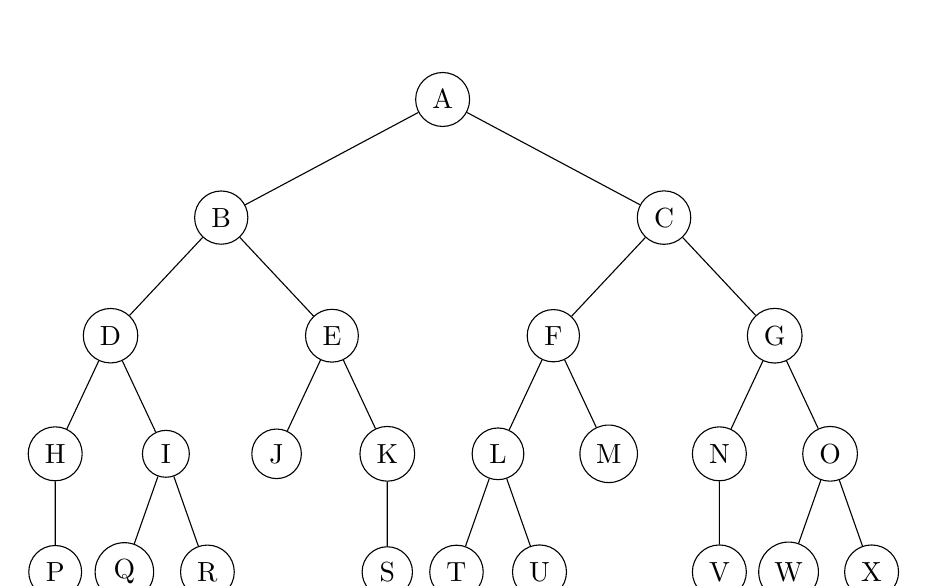
\begin{tikzpicture}
    [level 1/.style={sibling distance=16em},
      level 2/.style={sibling distance=8em},
      level 3/.style={sibling distance=4em},
      level 4/.style={sibling distance=3em}
    ]
    \node [circle,draw] {A}
    child {node [circle,draw] {B}
        child {node [circle,draw] {D}
            child {node [circle,draw] {H}
                child {node [circle,draw] {P}}
              }
            child {node [circle,draw] {I}
                child {node [circle,draw] {Q}}
                child {node [circle,draw] {R}}
              }
          }
        child {node [circle,draw] {E}
            child {node [circle,draw] {J}}
            child {node [circle,draw] {K}
                child {node [circle,draw] {S}}
              }
          }
      }
    child {node [circle,draw] {C}
        child {node [circle,draw] {F}
            child {node [circle,draw] {L}
                child {node [circle,draw] {T}}
                child {node [circle,draw] {U}}
              }
            child {node [circle,draw] {M}
              }
          }
        child {node [circle,draw] {G}
            child {node [circle,draw] {N}
                child {node [circle,draw] {V}}
              }
            child {node [circle,draw] {O}
                child {node [circle,draw] {W}}
                child {node [circle,draw] {X}}
              }
          }
      }
    ;
  \end{tikzpicture}
\end{center}

\begin{qparts}
  \item (3 points) Write out the order that the nodes are expanded in using Breadth First Search, starting from A and searching to N.\\
  \textcolor{blue}{A B C D E F G H I J K L M N}
  \item (3 points) Write out the order that the nodes are expanded in using Depth First Search, starting from A and searching to N.\\
  \textcolor{blue}{A B D H P I Q R E J K S C F L T U M G N}
  \item (3 points) Write out the order that the nodes are expanded in using Iterative-Deepening Depth First Search, starting from A and searching to N. If a node is repeated, make sure to include it each time it is expanded.\\
  \textcolor{blue}{A A B C A B D E C F G A B D H I E J K C F L M G N}
  \item (4 points) Which of the three search algorithms (BFS, DFS, IDDFS) has the smallest maximum size of the open list while searching from A to K? What is the maximum size of the open list for that algorithm?\\
  \textcolor{blue}{The search algorithm with the smallest maximum size of the open list is IDDFS with a maximum size of 4 searching from A to K}
  \item (2 points) True or False: BFS, DFS, and IDDFS will each return the same path on this tree starting at A searching to K.\\
  \textcolor{blue}{True}
  \item (2 points) True or False: Given the same start and goal state, BFS, DFS, and IDDFS will always return the same path for any search graph (not necessarily a tree).\\
  \textcolor{blue}{False}
  \item (4 points) Suppose you are running your search algorithm on an embedded system device with highly limited memory available. Which of the three search algorithms (BFS, DFS, IDDFS) would you choose to run to minimize the memory used by the algorithm? Justify your answer with a one sentence explanation.\\
  \textcolor{blue}{IDDFS because IDDFS only needs to store the nodes of the tree at the current depth, then discards them when it is time to move to the next iteration of the call.}
  \item (4 points) Suppose you need to run a search algorithm but you are confident that the vast majority of your search goals will be near the root of the tree (for example, G or earlier in the alphabet on this tree). Which of the three search algorithms (BFS, DFS, IDDFS) would you use to find the shortest path in the least amount of time given these conditions? Justify your answer with a one sentence explanation.\\
  \textcolor{blue}{BFS because it is more time-efficient than DFS at finding nodes higher in the tree on average, and IDDFS' advantage over BFS is the memory, which is not of concern. }
\end{qparts}

\newpage
%-----------------------------------------------------
\section{Heuristic Search}
\begin{center}
  \tikz {
    \node [circle,draw] (S)              {S};
    \node [circle,draw] (f) [above=of S] {f};
    \node [circle,draw] (a) [right=of S] {a};
    \node [circle,draw] (b) [below=of a] {b};
    \node [circle,draw] (c) [right=of b] {c};
    \node [circle,draw] (e) [right=of a] {e};
    \node [circle,draw] (d) [above=of e] {d};
    \node [circle,draw] (G) [right=of e] {G};

    \draw [->]
    (S) edge["1"]   (f)
    (S) edge["1"]   (a)
    (S) edge["3"]   (b)
    (a) edge["2"]   (d)
    (b) edge["1"]   (c)
    (c) edge["2"]   (e)
    (d) edge["2"]   (e)
    (a) edge["2"]   (b)
    (c) edge["5"]   (G)
    (e) edge["2"]   (G)

  }
\end{center}

For the following questions, consider three heuristics $h_1$, $h_2$, $h_3$. The table below indicates the estimated cost to goal, $G$, for each of the heuristics for each node in the search graph.
\begin{center}
  \begin{tabular}{||c c c c c c c c c||}
    \hline
    state (s)          & S & a & b & c & d & e & f & G \\ [0.5ex]
    \hline\hline
    heuristic $h_1(s)$ & 6 & 5 & 2 & 2 & 2 & 2 & 6 & 0 \\
    \hline
    heuristic $h_2(s)$ & 6 & 6 & 4 & 5 & 4 & 1 & 5 & 0 \\
    \hline
    heuristic $h_3(s)$ & 6 & 6 & 4 & 3 & 4 & 2 & 8 & 0 \\
    \hline
  \end{tabular}
\end{center}

\begin{qparts}
  \item (2 point)
  What does it mean for a heuristic to be "admissible"? \\
  \textcolor{blue}{A heuristic is admissible when the estimated cost it provides to the reach the goal node is never higher than the actual cost to reach the goal node, for any goal state and for any starting node.}

  \item (3 points)
  Which heuristics among $\{h_1, h_2, h_3\}$ shown above
  are admissible? For heuristics which are not admissible,
  please identify the nodes where admissibility is violated. \\
  \textcolor{blue}{Heuristics $\{h_1, h_3\}$ are admissible. Admissibility is violated in $h_2$ at node $c$}


  \item (2 point)
  What does it mean for a heuristic to be "consistent"? \\
  \textcolor{blue}{A heuristic is consistent when, for each edge connecting two nodes, the difference of the heuristic value between the two nodes is never greater than the true distance between the two nodes.}


  \item (3 points)
  Which heuristics are consistent?
  For heuristics which are not consistent,
  please identify the edges where consistency is violated.\\
  \textcolor{blue}{Heuristic $h_3$ is consistent. $h_1$ violates consistency at edges $\{(S, b), (a, d), (a, b)\}$.
    $h_2$ violates consistency at edges $\{(c, e), (d, e)\}$.}

  \item (2 points) What does it mean for one heuristic to
  dominate another heuristic?\\
  \textcolor{blue}{A heuristic dominates another when the heuristic value for all nodes for one function is greater than the heuristic value for all nodes in the other. We assume that both heuristics are admissible.}

  \item (2 points) Of the heuristics provided above,
  which would you consider the best heuristic?
  Explain your reasoning in terms of admissibility,
  consistency, and dominance.\\
  \textcolor{blue}{Heuristic $h_3$ is the best heuristic because it is the only heuristic that is both admissible and consistent. It also dominates $h_1$, the only other heuristic that is admissible.}

  \item  (4 points)
  Show the node expansion order going from S to G using $A*$
  with the heuristic you identified in the previous question.
  Also provide the final (solution) path obtained. \\
  \textcolor{blue}{Node expansion path: $S, a, b, d, c, e, G$. The final path is $S, a, d, e, g$.}

  \item (1 points) Consider $h_1$ -- what single change would
  you make to improve this heuristic? \\
  \textcolor{blue}{I would change $h(a)$ to equal 4, rather than 5.}
  \item (4 points) Having made the change above,
  has your determination of the best heuristic changed?
  Explain your reasoning in terms of admissibility, consistency,
  and dominance.\\
  \textcolor{blue}{This change would keep the heuristic admissible, but improve its consistency. The edges $\{(a, d), (a, b)\}$ would become consistent. Edge $(S, b)$ would remain not-consistent, but since that edge is not used in the shortest path, it would not be important. The heuristic would remain dominated by $h_3$, but I believe this is the best single change to improve $h_1$. Full consistency could be achived by also decreasing the value of $h(s)$ by one.}


  \item (2 points)  Explain why, when using the $A*$ search algorithm,
  it is important to continue the expansion process until
  the goal state is removed from the OPEN list and becomes
  the current state, rather than terminating as soon as the GOAL state is found.\\
  \textcolor{blue}{The priority value of the goal state can be updated by other nodes being expanded. If other nodes have not had the chance to update the goal nodes priority, then the shortest path has not been found. A path has been found, but possibly not the shortest.}
\end{qparts}


\newpage
%-----------------------------------------------------
\section{Adversarial Search and Alpha-Beta Pruning}

\subsection{Alpha-Beta Pruning}
Use this search tree along with the table of state
evaluation values to answer the questions below.
By default, children are processed from left to right.

\begin{center}
  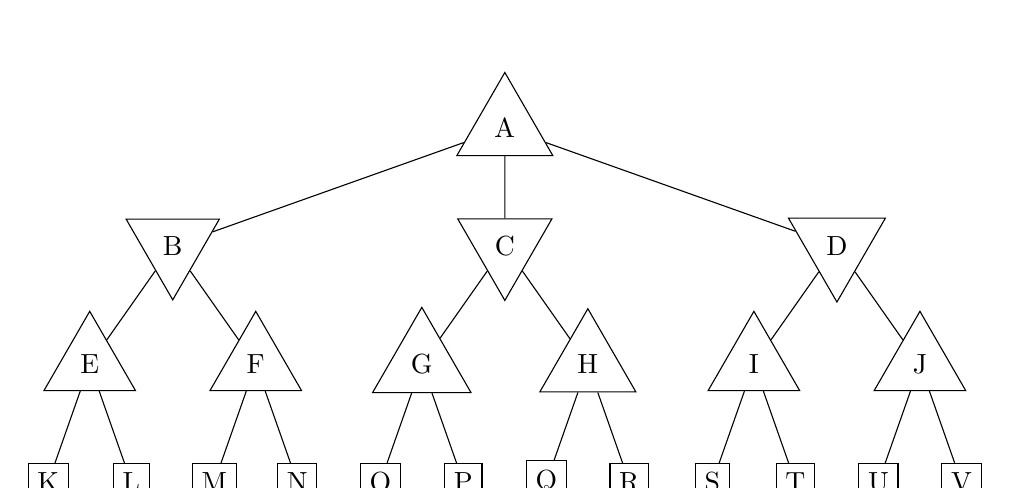
\begin{tikzpicture}
    [level 1/.style={sibling distance=12em},
      level 2/.style={sibling distance=6em},
      level 3/.style={sibling distance=3em},
    ]
    \node [regular polygon, regular polygon sides=3, shape border rotate=0,draw] {A}
    child {node [regular polygon, regular polygon sides=3, shape border rotate=180,draw] {B}
        child {node [regular polygon, regular polygon sides=3, shape border rotate=0,draw] {E}
            child {node [draw] {K}}
            child {node [draw] {L}}
          }
        child {node [regular polygon, regular polygon sides=3, shape border rotate=0,draw] {F}
            child {node [draw] {M}}
            child {node [draw] {N}}
          }
      }
    child {node [regular polygon, regular polygon sides=3, shape border rotate=180,draw] {C}
        child {node [regular polygon, regular polygon sides=3, shape border rotate=0,draw] {G}
            child {node [draw] {O}}
            child {node [draw] {P}}
          }
        child {node [regular polygon, regular polygon sides=3, shape border rotate=0,draw] {H}
            child {node [draw] {Q}}
            child {node [draw] {R}}
          }
      }
    child {node [regular polygon, regular polygon sides=3, shape border rotate=180,draw] {D}
        child {node [regular polygon, regular polygon sides=3, shape border rotate=0,draw] {I}
            child {node [draw] {S}}
            child {node [draw] {T}}
          }
        child {node [regular polygon, regular polygon sides=3, shape border rotate=0,draw] {J}
            child {node [draw] {U}}
            child {node [draw] {V}}
          }
      }
    ;
  \end{tikzpicture}
\end{center}

\begin{table}[H]
  \centering
  \begin{tabular}{|l|l|l|l|l|l|l|l|l|l|l|l|l|}
    \hline
    state      & K & L  & M & N & O  & P  & Q & R  & S & T  & U & V \\ \hline
    evaluation & 5 & -3 & 6 & 8 & -3 & -5 & 6 & -4 & 9 & -5 & 2 & 1 \\ \hline
  \end{tabular}
\end{table}

\begin{qparts}
  \item (8 points) Use minimax to perform adversarial search with alpha-beta pruning on the tree above. Fill in the values in the table below as you go. For $\alpha$ and $\beta$ values, write the values that are passed from the state's parent to that state. For example, the value of state K will not be shown in the $\alpha-\beta$ values of state E, but would be reflected in the $\alpha-\beta$ values of state L. If a state does not have to be evaluated, do not write any values for it in the table.

  \begin{table}[t]
    \begin{center}
      \begin{tabular}{|l|m{5em}|m{5em}|m{5em}|}
        \hline
        state & value & $\alpha$  & $\beta$  \\ \hline
        A     & 5     & N/A       & N/A      \\ \hline
        B     & 5     & $-\infty$ & $\infty$ \\ \hline
        C     & -3    & 5         & $\infty$ \\ \hline
        D     & 2     & 5         & $\infty$ \\ \hline
        E     & 5     & $-\infty$ & $\infty$ \\ \hline
        F     & 6     & $-\infty$ & 5        \\ \hline
        G     & -3    & 5         & $\infty$ \\ \hline
        H     &       &           &          \\ \hline
        I     & 9     & 5         & $\infty$ \\ \hline
        J     & 2     & 5         & 9        \\ \hline
        K     & 5     & $-\infty$ & $\infty$ \\ \hline
        L     & -3    & 5         & $\infty$ \\ \hline
        M     & 6     & $-\infty$ & 5        \\ \hline
        N     & 8     &           &          \\ \hline
        O     & -3    & 5         & $\infty$ \\ \hline
        P     & -5    & 5         & $\infty$ \\ \hline
        Q     & 6     &           &          \\ \hline
        R     & -4    &           &          \\ \hline
        S     & 9     & 5         & $\infty$ \\ \hline
        T     & -5    & 9         & $\infty$ \\ \hline
        U     & 2     & 5         & 9        \\ \hline
        V     & 1     & 5         & 2        \\ \hline
      \end{tabular}
    \end{center}
  \end{table}
  \item (7 points) Let’s assume that you \st{reverse} {\em change} the order of the leaf nodes in the above tree A (call that \st{reversed} tree B). The evaluation function f represents the utilities for the first tree A, and let the evaluation function g represent the utilities for the second tree B. \st{After performing alpha beta on this reversed tree, what observations can you make about the two evaluation functions? Be sure to answer what effect switching the order of the evaluation function utilities has.  What are some ways to improve the evaluation functions in general?}

  {\em Is it possible to completely prevent pruning in the tree by just reordering the leaf nodes in the tree? If so, explain why. If not, what is the least number of leaf nodes whose values need to be changed to prevent pruning. In either case, describe your new tree.
    (Include a drawing if you think it will be more clear that way.)} \\
  \textcolor{blue}{Two leaf node values must be changed. A possible reordering of the leaves that would result in no pruning of the tree is as follows (assuming leaf nodes can only be reordered under their parent leaf node as is stated on ed thread 163):} \\
  \begin{table}[H]
    \centering
    \begin{tabular}{|l|l|l|l|l|l|l|l|l|l|l|l|l|}
      \hline
      state      & K & L  & M  & N & O & P  & Q & R  & S & T  & U & V \\ \hline
      evaluation & 5 & -3 & -4 & 8 & 6 & -5 & 5 & -4 & 9 & -5 & 2 & 1 \\ \hline
    \end{tabular}
  \end{table}
  \textcolor{blue}{This reordering was found by decreasing the value of node M to a value less than the beta value passed to it, and increasing node O to a value greater than the beta value passed to it, and switching nodes Q and R. Since switching nodes under the first E and F does not occur in avoiding pruning, value N must be changed to avoid pruning. By increasing the value of node O, we avoid the pruning of everything to the right of node C. But in that case, node R still is pruned. We avoid this by switching Q and R since we need node Q to have a value less than the beta value passed to it.}
\end{qparts}

\subsection{Pruning with Chance Nodes}

Although alpha-beta pruning cannot be applied directly to searching trees that contain chance nodes, reasoning like that inherent in alpha-beta search can sometimes be applied when static values are constrained to lie within given ranges of values.
For example, if all leaf-node values must be values $f(s)$ such that\
$ 0 \le f(s) \le 10$, then node G can be pruned in the tree below,
because Max can get 9 by moving left at A to B, and
if Max goes to C and finds $f(F)=3$, Max can reason that getting $f(G)$ is
useless because if $f(G)=10$ which is largest allowed, then the value at C is (3+10)/2 = 6.5, which is inferior to 9.

\begin{center}
  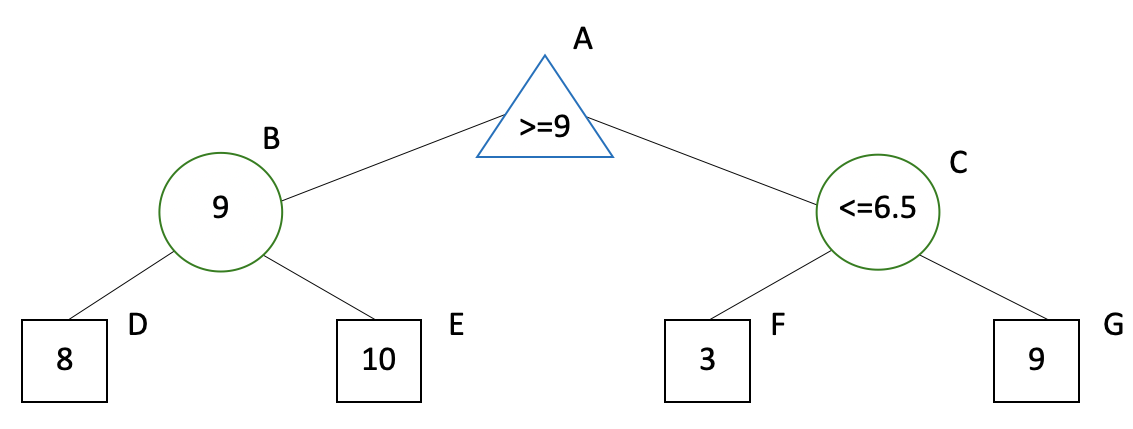
\includegraphics[width=6in]{q3-Expectimax-Pruning-Example.png}
\end{center}

\begin{qparts}
  \setcounter{enumi}{2}
  \item (6 points) In the following game tree, determine where pruning can be performed
  using the same range assumption as above.  Show where there are cutoffs. Also after pruning, change the value of one of the nodes such that the pruning will no longer occur.\\
  \textcolor{blue}{Pruning will occur at node k. If node j is changed to a value less than node i, then pruning will not occur at node k. Pruning will also occur at node g. If node m is changes to 0, then pruning will not occur at node g.}
  \item (4 points) Explain your reasoning for each cutoff.\\
  \textcolor{blue}{Pruning will occur at node k because of regular alpha-beta pruning behavior. Pruning will occur at node g because since node m is of value 10, the average value that will be passed up to node c will be greater than 5, meaning that the minimizing head node will go to b since the average value there will be 4.}
  \begin{center}
    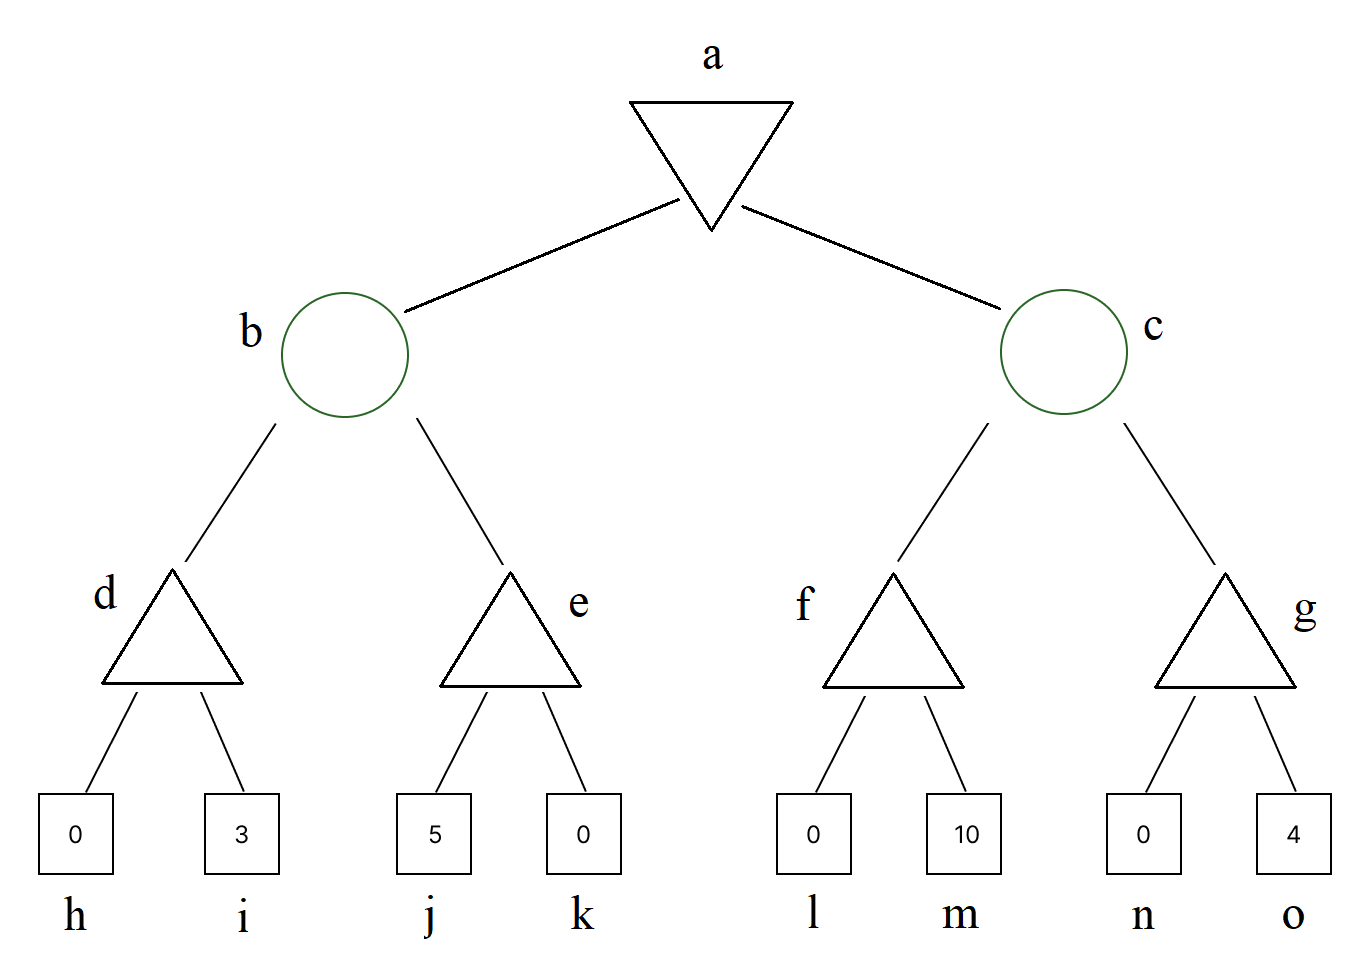
\includegraphics[width=6in]{q3-Pruning-with-Chance-Nodes.png}
  \end{center}

\end{qparts}
\newpage
%-----------------------------------------------------
\section{Probabilistic Inference and Factoring Joint Distributions}

\begin{qparts}


  \item (10 points) Consider a situation where we are modeling the sale of Ice cream (S), which is dependent on three variables: Weather condition (W) and Day of the week (D). You are given the joint probability distribution of these variables in the table below:

  \begin{table}[h]
    \centering
    \begin{tabular}{|c|c|c|c|}
      \hline
      Weather (W) & Day (D)      & Ice Cream Sales (S) & P(W,D,S) \\ \hline \hline
      Sunny (Su)  & Weekday (Wd) & High                & 0.108    \\ \hline
      Sunny (Su)  & Weekday (Wd) & Low                 & 0.252    \\ \hline
      Sunny (Su)  & Weekend (We) & High                & 0.216    \\ \hline
      Sunny (Su)  & Weekend (We) & Low                 & 0.024    \\ \hline
      Cloudy (Cl) & Weekday (Wd) & High                & 0.024    \\ \hline
      Cloudy (Cl) & Weekday (Wd) & low                 & 0.096    \\ \hline
      Cloudy (Cl) & Weekend (We) & High                & 0.032    \\ \hline
      Cloudy (Cl) & Weekend (We) & Low                 & 0.048    \\ \hline
      Rainy (Ra)  & Weekday (Wd) & High                & 0.012    \\ \hline
      Rainy (Ra)  & Weekday (Wd) & Low                 & 0.108    \\ \hline
      Rainy (Ra)  & Weekend (We) & High                & 0.016    \\ \hline
      Rainy (Ra)  & Weekend (We) & Low                 & 0.064    \\ \hline
      \hline
    \end{tabular}
    \caption{Joint Probability Distribution of Weather, Day, and Ice Cream Sales. }
    \label{tab:my_label}
  \end{table}

  Answer these questions based on the joint probability distribution table above:
  \begin{qsubparts}
    \item What is the marginal distribution  P(W) ?\\
    \begin{table}[h]
      \centering
      \begin{tabular}{|c|c|c|c|}
        \hline
        Weather (W) & P(W) \\ \hline \hline
        Sunny (Su)  & 0.6  \\ \hline

        Cloudy (Cl) & 0.2  \\ \hline

        Rainy (Ra)  & 0.2  \\ \hline

        \hline
      \end{tabular}
      \label{tab:my_label_1}
    \end{table} \\ \\ \\ \\ \\ \\ \\ \\ \\ \\
    \item What is the marginal distribution  P(W, D) ?
    \begin{table}[h]
      \centering
      \begin{tabular}{|c|c|c|c|}
        \hline
        Weather (W) & Day (D)      & P(W,D) \\ \hline \hline
        Sunny (Su)  & Weekday (Wd) & 0.36   \\ \hline
        Sunny (Su)  & Weekend (We) & 0.24   \\ \hline
        Cloudy (Cl) & Weekday (Wd) & 0.12   \\ \hline
        Cloudy (Cl) & Weekend (We) & 0.08   \\ \hline
        Rainy (Ra)  & Weekday (Wd) & 0.12   \\ \hline
        Rainy (Ra)  & Weekend (We) & 0.08   \\ \hline
        \hline
      \end{tabular}
      \label{tab:my_label_2}
    \end{table}

    \item What is the marginal distribution  P(W, S) ?
    \begin{table}[h]
      \centering
      \begin{tabular}{|c|c|c|c|}
        \hline
        Weather (W) & Ice Cream Sales (S) & P(W,S) \\ \hline \hline
        Sunny (Su)  & High                & 0.324  \\ \hline
        Sunny (Su)  & Low                 & 0.276  \\ \hline
        Cloudy (Cl) & High                & 0.056  \\ \hline
        Cloudy (Cl) & low                 & 0.144  \\ \hline
        Rainy (Ra)  & High                & 0.028  \\ \hline
        Rainy (Ra)  & Low                 & 0.172  \\ \hline
        \hline
      \end{tabular}
      \label{tab:my_label_4}
    \end{table}



    \item What is the marginal distribution  P(D) ?
    \begin{table}[h]
      \centering
      \begin{tabular}{|c|c|c|c|}
        \hline
        Day (D)      & P(D) \\ \hline \hline
        Weekday (Wd) & 0.6  \\ \hline
        Weekend (We) & 0.4  \\ \hline

        \hline
      \end{tabular}
      \label{tab:my_label}
    \end{table}
    \newpage

    \item What is the conditional distribution  P(S $|$ W, D)?
    \begin{table}[h]
      \centering
      \begin{tabular}{|c|c|c|c|}
        \hline
        Weather (W) & Day (D)      & Ice Cream Sales (S) & P(S$|$W,D) \\ \hline \hline
        Sunny (Su)  & Weekday (Wd) & High                & 0.108/0.36 \\ \hline
        Sunny (Su)  & Weekday (Wd) & Low                 & 0.252/0.36 \\ \hline
        Sunny (Su)  & Weekend (We) & High                & 0.216/0.24 \\ \hline
        Sunny (Su)  & Weekend (We) & Low                 & 0.024/0.24 \\ \hline
        Cloudy (Cl) & Weekday (Wd) & High                & 0.024/0.12 \\ \hline
        Cloudy (Cl) & Weekday (Wd) & low                 & 0.096/0.12 \\ \hline
        Cloudy (Cl) & Weekend (We) & High                & 0.032/0.08 \\ \hline
        Cloudy (Cl) & Weekend (We) & Low                 & 0.048/0.08 \\ \hline
        Rainy (Ra)  & Weekday (Wd) & High                & 0.012/0.12 \\ \hline
        Rainy (Ra)  & Weekday (Wd) & Low                 & 0.108/0.12 \\ \hline
        Rainy (Ra)  & Weekend (We) & High                & 0.016/0.08 \\ \hline
        Rainy (Ra)  & Weekend (We) & Low                 & 0.064/0.08 \\ \hline
        \hline
      \end{tabular}
      \label{tab:my_label_5}
    \end{table}
  \end{qsubparts}
  \newpage
  \vspace{5em}

  \begin{center}
    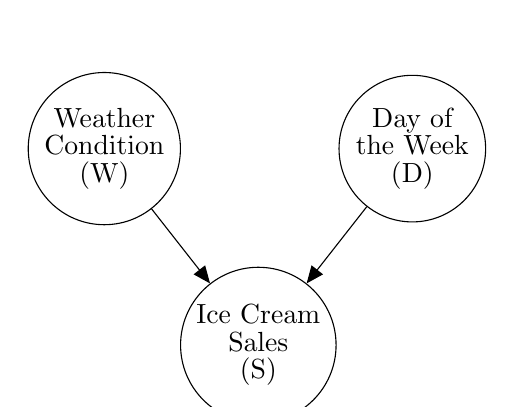
\begin{tikzpicture}
      \node[latent, align=center] (weather) {Weather \\ Condition\\ (W)};
      \node[latent, align=center, right=2cm of weather] (day) {Day of \\ the Week\\ (D)};
      \node[latent, align=center, below=1.5cm of $(weather)!0.5!(day)$] (sales) {Ice Cream \\ Sales\\ (S)};

      % Edges
      \draw[->] (weather) -- (sales);
      \draw[->] (day) -- (sales);
    \end{tikzpicture}
  \end{center}

  \item (6 points) Consider the Bayes Net of the same Ice Cream Sales problem we were considering. Answer the following question based on it:
  \begin{qsubparts}
    \item Write the equation for the joint distribution of the three variables as a product of the appropriate marginal and conditional distributions, according to the Bayes net graph.\\
    \textcolor{blue}{$P(W,D,S) = P(W)*P(D)*P(S|W,D)$}
    \item What is the probability of high ice cream sales on a weekend, given that the weather is sunny?\\
    \textcolor{blue}{P(S=h $\mid$ D=We,W=s) = P(W=s,D=We,S=h)/(P(W=s)*P(D=We))\\ = $\frac{0.216}{0.6*0.4}$}
    \item Given that ice cream sales are high, what is the probability that the day is a weekend?\\
    \textcolor{blue}{P(Weekend $\mid$ High) = $\frac{0.264}{0.6}$}
    \item What is the probability of having a sunny weekday with high ice cream sales compared to having a rainy weekend with low ice cream sales?\\
    \textcolor{blue}{$P(W = sunny, D = weekday, S = high) = P(W = sunny)P(D = weekday)P(S = high|W = sunny, D = weekday)$}\\
    \textcolor{blue}{$= 0.6 * 0.6 * \frac{0.108}{0.408} = 0.095$}\\
    \textcolor{blue}{$P(W = rainy, D = weekend, S = low) = P(W = rainy)P(D = weekend)P(S = low|W = rainy, D = weekend)$}\\
    \textcolor{blue}{$= 0.4 * 0.4 * \frac{0.064}{0.052} = 0.197$}
  \end{qsubparts}
  \newpage
  \item (9 points) Compare the sizes of the representations for the full joint distribution in (a)
  and the Bayes net in (b) as follows:
  \begin{qsubparts}
    \item
    Give an expression for the number of free parameters in Table 1 in terms of the
    sizes of the domains of the variables W, D, and S.  You can use $|W|$ to represent
    the size of the domain of W, for example.\\
    \textcolor{blue}{number of free parameters = $|W|*|D|*|S| - 1$}

    \item Give the resulting integer value for your expression.\\
    \textcolor{blue}{$11$}

    \item Give a corresponding expression for the number of free parameters in the
    Bayes net in (b).\\
    \textcolor{blue}{Number of free parameters = $|W|-1 + |D|-1 + |W|*|D|*(|S|-1)$}
    \item Give the integer value of the expression for the Bayes net.\\
    \textcolor{blue}{$2 + 1 + 3*2*(2-1) = 9$}
    \item Is there any savings in storage, according to the number of free parameters?
    Explain.\\
    \textcolor{blue}{Since bayes nets' exploit conditional independance among the variables in the distribution to reduce the number of free parameters, there is infact a saving in storage when comparing the bayes net to the full joint distribution.}

    \item What kind of changes to this joint distribution and Bayes net could lead to a significant savings?\\
    \textcolor{blue}{Increasing the number of variables and the sizes of their domains would have saving by decreasing the number of free parameters in relation to the full joint distribution that these changes would cause.}
  \end{qsubparts}
\end{qparts}

\end{document}
